\documentclass[aspectratio=169]{beamer}

% Theme
\usetheme{default}
\usecolortheme{beaver}

% Packages
\usepackage{amsmath,amssymb,amsthm}
\usepackage{mathtools}
\usepackage{bm}
\usepackage{tikz}
\usetikzlibrary{arrows.meta,positioning,calc,patterns,decorations.markings,shapes}

% Custom commands
\newcommand{\R}{\mathbb{R}}
\newcommand{\Z}{\mathbb{Z}}
\newcommand{\Pp}{\mathcal{P}}
\newcommand{\Hone}{\mathcal{H}^1}

% Title
\title{Counter-examples to Existence}
\subtitle{When Optimal Transport Maps Fail}
\author{}
\date{}

\begin{document}

%==============================================================================
\begin{frame}
\titlepage
\end{frame}

%==============================================================================
\begin{frame}{Outline}
\tableofcontents[hideallsubsections]
\end{frame}

%==============================================================================
\section{Counter-examples to Existence}
%==============================================================================

\begin{frame}{When Do Optimal Maps Fail to Exist?}
\textbf{Recall Theorem 1.17:} Under certain conditions (twist condition, $\mu \ll \mathcal{L}^d$), an optimal transport \emph{map} exists.

\vspace{0.4cm}
\textbf{Question:} What happens when these conditions are violated?

\vspace{0.4cm}
\textbf{Focus:} We examine cases where the cost $c(x,y)$ would normally allow existence (e.g., $c(x,y) = |x-y|^2$), but the \textbf{source measure} $\mu$ causes problems.

\vspace{0.4cm}
\textbf{Two types of failure:}
\begin{enumerate}
    \item No transport map exists at all
    \item Transport maps exist, but none is optimal
\end{enumerate}
\end{frame}

%==============================================================================
\begin{frame}{Example 1: No Transport Map Exists}
\begin{columns}
\begin{column}{0.55\textwidth}
\textbf{Setup:} Let $\mu = \delta_a$ for some $a \in X$.

Suppose $\nu$ is \textbf{not} a Dirac mass.

\vspace{0.3cm}
\textbf{Key observation:}
\[
\boxed{T_\# \delta_a = \delta_{T(a)}}
\]

\textbf{Proof:} For any set $B$:
\[
(T_\# \delta_a)(B) = \delta_a(T^{-1}(B)) = \begin{cases} 1 & T(a) \in B \\ 0 & T(a) \notin B \end{cases}
\]

\vspace{0.3cm}
$\Rightarrow$ \textbf{No transport map} $T: X \to Y$ can exist if $\nu \neq \delta_b$ for some $b \in Y$.
\end{column}
\begin{column}{0.45\textwidth}
\begin{center}
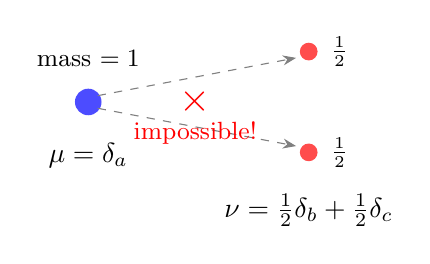
\begin{tikzpicture}[scale=0.8]
    % Source: Dirac mass
    \fill[blue!70] (0,0) circle (6pt);
    \node[below] at (0,-0.5) {$\mu = \delta_a$};
    \node[above, font=\small] at (0,0.4) {mass $= 1$};

    % Target: two points
    \fill[red!70] (3.5,0.8) circle (4pt);
    \node[right, font=\small] at (3.7,0.8) {$\frac{1}{2}$};
    \fill[red!70] (3.5,-0.8) circle (4pt);
    \node[right, font=\small] at (3.7,-0.8) {$\frac{1}{2}$};
    \node[below] at (3.5,-1.3) {$\nu = \frac{1}{2}\delta_b + \frac{1}{2}\delta_c$};

    % Impossible arrows
    \draw[-{Stealth},gray,dashed] (0.15,0.1) -- (3.3,0.7);
    \draw[-{Stealth},gray,dashed] (0.15,-0.1) -- (3.3,-0.7);

    % X mark
    \node[red,font=\Large] at (1.7,0) {\textbf{$\times$}};

    % Caption
    \node[red, font=\small] at (1.7,-0.5) {impossible!};
\end{tikzpicture}

\vspace{0.3cm}
\textbf{A map cannot split mass!}
\end{center}
\end{column}
\end{columns}
\end{frame}

%==============================================================================
\begin{frame}{Why Atoms Are Problematic}
\textbf{General principle:} The image measure $T_\# \mu$ always includes an atom of mass at least $\mu(\{a\})$ for every atom $a$ of $\mu$.

\vspace{0.4cm}
\textbf{Consequence:}
\begin{itemize}
    \item Measures with atoms \textbf{cannot} be transported via maps to measures without atoms
    \item The absence of atoms is a \textbf{typical assumption} on $\mu$ when solving (MP)
\end{itemize}

\vspace{0.4cm}
\begin{center}
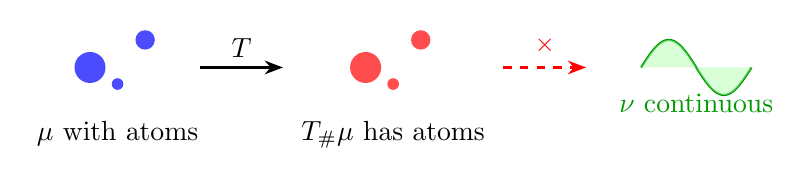
\begin{tikzpicture}[scale=0.7]
    % Atomic measure
    \fill[blue!70] (0,0) circle (8pt);
    \fill[blue!70] (1,0.5) circle (5pt);
    \fill[blue!70] (0.5,-0.3) circle (3pt);
    \node[below] at (0.5,-0.8) {$\mu$ with atoms};

    \draw[-{Stealth},thick] (2,0) -- node[above] {$T$} (3.5,0);

    % Image measure
    \fill[red!70] (5,0) circle (8pt);
    \fill[red!70] (6,0.5) circle (5pt);
    \fill[red!70] (5.5,-0.3) circle (3pt);
    \node[below] at (5.5,-0.8) {$T_\#\mu$ has atoms};

    \draw[-{Stealth},thick,red,dashed] (7.5,0) -- (9,0);
    \node[red] at (8.25,0.4) {\small $\times$};

    % Continuous target
    \draw[green!60!black, thick] plot[smooth, domain=10:12] (\x, {0.5*sin((\x-10)*180)});
    \fill[green!30, opacity=0.5] plot[smooth, domain=10:12] (\x, {0.5*sin((\x-10)*180)}) -- (12,0) -- (10,0) -- cycle;
    \node[below, green!60!black] at (11,-0.3) {$\nu$ continuous};
\end{tikzpicture}
\end{center}
\end{frame}

%==============================================================================
\begin{frame}{Kantorovich Saves the Day}
\begin{columns}
\begin{column}{0.5\textwidth}
\textbf{Key insight:} The Kantorovich problem (KP) still makes sense for atomic measures!

\vspace{0.3cm}
\textbf{When $\mu = \delta_a$:}

The set $\Pi(\mu, \nu)$ contains a \textbf{unique} element:
\[
\boxed{\gamma = \mu \otimes \nu = \delta_a \otimes \nu}
\]

\vspace{0.3cm}
\textbf{Interpretation:}
\begin{itemize}
    \item All mass starts at $a$
    \item Distributes to $\nu$ according to product structure
    \item Mass \textbf{can split} in Kantorovich!
\end{itemize}
\end{column}
\begin{column}{0.5\textwidth}
\begin{center}
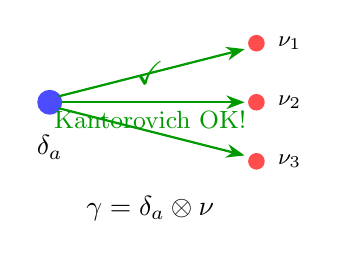
\begin{tikzpicture}[scale=0.75]
    % Source
    \fill[blue!70] (0,0) circle (6pt);
    \node[below] at (0,-0.4) {$\delta_a$};

    % Targets
    \fill[red!70] (3.5,1) circle (4pt);
    \fill[red!70] (3.5,0) circle (4pt);
    \fill[red!70] (3.5,-1) circle (4pt);
    \node[right, font=\footnotesize] at (3.7,1) {$\nu_1$};
    \node[right, font=\footnotesize] at (3.7,0) {$\nu_2$};
    \node[right, font=\footnotesize] at (3.7,-1) {$\nu_3$};

    % Kantorovich arrows (splitting OK)
    \draw[-{Stealth},green!60!black,thick] (0.15,0.1) -- (3.3,0.9);
    \draw[-{Stealth},green!60!black,thick] (0.2,0) -- (3.3,0);
    \draw[-{Stealth},green!60!black,thick] (0.15,-0.1) -- (3.3,-0.9);

    % Checkmark
    \node[green!60!black,font=\large] at (1.7,0.5) {\checkmark};

    % Label
    \node[green!60!black, font=\small] at (1.7,-0.3) {Kantorovich OK!};

    % Plan formula
    \node at (1.7,-1.8) {$\gamma = \delta_a \otimes \nu$};
\end{tikzpicture}
\end{center}
\end{column}
\end{columns}
\end{frame}

%==============================================================================
\begin{frame}{Example 2: Setup --- Three Parallel Segments}
\textbf{Setup:} Consider three vertical parallel segments in $\R^2$:

\vspace{0.2cm}
\begin{columns}
\begin{column}{0.45\textwidth}
\begin{itemize}
    \item Segment $A$: at $x = 0$
    \item Segment $B$: at $x = 1$
    \item Segment $C$: at $x = -1$
\end{itemize}

All segments have vertices on lines $y = 0$ and $y = 1$.

\vspace{0.3cm}
\textbf{Cost function:}
\[
c(x,y) = |x - y|^2
\]
(quadratic cost)
\end{column}
\begin{column}{0.55\textwidth}
\begin{center}
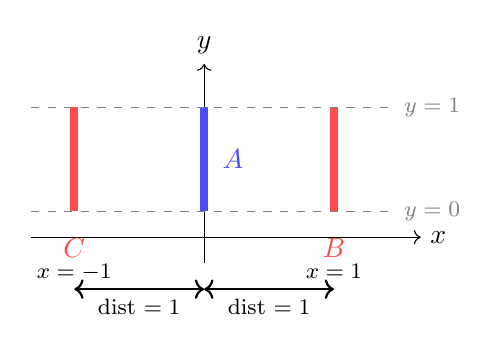
\begin{tikzpicture}[scale=1.1]
    % Coordinate axes
    \draw[->] (-2,0) -- (2.5,0) node[right] {$x$};
    \draw[->] (0,-0.3) -- (0,2) node[above] {$y$};

    % Segment C (left, x=-1)
    \draw[red!70, line width=3pt] (-1.5,0.3) -- (-1.5,1.5);
    \node[red!70, below] at (-1.5,0.1) {$C$};
    \node[below, font=\footnotesize] at (-1.5,-0.2) {$x=-1$};

    % Segment A (center, x=0)
    \draw[blue!70, line width=3pt] (0,0.3) -- (0,1.5);
    \node[blue!70, right] at (0.1,0.9) {$A$};

    % Segment B (right, x=1)
    \draw[red!70, line width=3pt] (1.5,0.3) -- (1.5,1.5);
    \node[red!70, below] at (1.5,0.1) {$B$};
    \node[below, font=\footnotesize] at (1.5,-0.2) {$x=1$};

    % Horizontal lines
    \draw[gray, dashed] (-2,0.3) -- (2.2,0.3);
    \node[gray, right, font=\footnotesize] at (2.2,0.3) {$y=0$};
    \draw[gray, dashed] (-2,1.5) -- (2.2,1.5);
    \node[gray, right, font=\footnotesize] at (2.2,1.5) {$y=1$};

    % Distance annotations
    \draw[<->, thick] (-1.5,-0.6) -- node[below, font=\footnotesize] {dist $=1$} (0,-0.6);
    \draw[<->, thick] (0,-0.6) -- node[below, font=\footnotesize] {dist $=1$} (1.5,-0.6);
\end{tikzpicture}
\end{center}
\end{column}
\end{columns}
\end{frame}

%==============================================================================
\begin{frame}{Example 2: The Measures}
\begin{columns}
\begin{column}{0.5\textwidth}
\textbf{Source measure:}
\[
\mu = \Hone \llcorner A
\]
($\Hone$ = 1-dimensional Hausdorff measure)

\vspace{0.3cm}
\textbf{Target measure:}
\[
\nu = \frac{\Hone \llcorner B + \Hone \llcorner C}{2}
\]
(half on $B$, half on $C$)
\end{column}
\begin{column}{0.5\textwidth}
\begin{center}
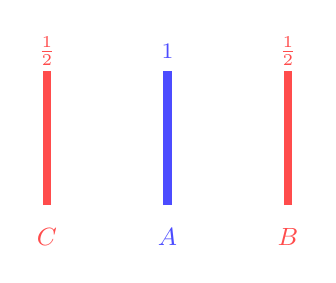
\begin{tikzpicture}[scale=0.85]
    % Segment C
    \draw[red!70, line width=3pt] (-1.8,0) -- (-1.8,2);
    \node[red!70, below, font=\small] at (-1.8,-0.2) {$C$};
    \node[red!70, font=\footnotesize] at (-1.8,2.3) {$\frac{1}{2}$};

    % Segment A
    \draw[blue!70, line width=3pt] (0,0) -- (0,2);
    \node[blue!70, below, font=\small] at (0,-0.2) {$A$};
    \node[blue!70, font=\footnotesize] at (0,2.3) {$1$};

    % Segment B
    \draw[red!70, line width=3pt] (1.8,0) -- (1.8,2);
    \node[red!70, below, font=\small] at (1.8,-0.2) {$B$};
    \node[red!70, font=\footnotesize] at (1.8,2.3) {$\frac{1}{2}$};
\end{tikzpicture}
\end{center}
\end{column}
\end{columns}
\end{frame}

%==============================================================================
\begin{frame}{Example 2: Why Cost $\geq 1$}
\textbf{Observation:} Every point on $A$ must move \textbf{horizontally} by distance $\geq 1$.

\vspace{0.3cm}
\begin{center}
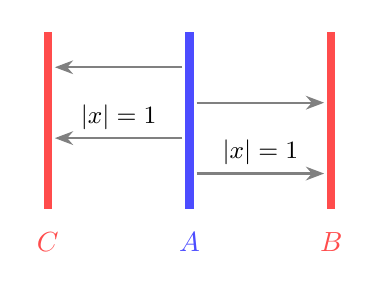
\begin{tikzpicture}[scale=0.9]
    % Segments
    \draw[red!70, line width=3pt] (-2,0) -- (-2,2.5);
    \node[red!70, below] at (-2,-0.2) {$C$};

    \draw[blue!70, line width=3pt] (0,0) -- (0,2.5);
    \node[blue!70, below] at (0,-0.2) {$A$};

    \draw[red!70, line width=3pt] (2,0) -- (2,2.5);
    \node[red!70, below] at (2,-0.2) {$B$};

    % Horizontal arrows showing minimum distance
    \draw[-{Stealth}, thick, gray] (0.1, 0.5) -- (1.9, 0.5);
    \draw[-{Stealth}, thick, gray] (0.1, 1.5) -- (1.9, 1.5);
    \draw[-{Stealth}, thick, gray] (-0.1, 1.0) -- (-1.9, 1.0);
    \draw[-{Stealth}, thick, gray] (-0.1, 2.0) -- (-1.9, 2.0);

    % Distance label
    \node[font=\small] at (1, 0.8) {$|x|=1$};
    \node[font=\small] at (-1, 1.3) {$|x|=1$};
\end{tikzpicture}
\end{center}

\vspace{0.3cm}
\textbf{Consequence:}
\[
\text{Cost} = \int |T(x) - x|^2 \, d\mu(x) \geq \int 1 \, d\mu = 1
\]

$\Rightarrow$ \textbf{No transport plan can achieve cost $< 1$}.
\end{frame}

%==============================================================================
\begin{frame}{Example 2: Approximating Maps $T_n$}
\textbf{Construction:}
\begin{itemize}
    \item Divide $A$ into $2n$ equal segments: $(A_i)_{i=1,\ldots,2n}$ (ordered downwards)
    \item Divide $B$ into $n$ segments: $(B_i)_{i=1,\ldots,n}$
    \item Divide $C$ into $n$ segments: $(C_i)_{i=1,\ldots,n}$
\end{itemize}

\vspace{0.2cm}
\textbf{Define $T_n$:} Piecewise affine map sending
\[
A_{2i-1} \to B_i \quad \text{and} \quad A_{2i} \to C_i
\]

\begin{center}
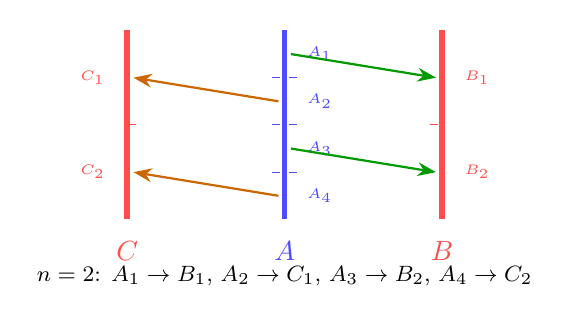
\begin{tikzpicture}[scale=0.8]
    % Segment C
    \draw[red!70, line width=2pt] (-2.5,0) -- (-2.5,3);
    \node[red!70, below] at (-2.5,-0.2) {$C$};
    \draw[red!70, dashed] (-2.5,1.5) -- (-2.3,1.5);
    \node[red!70, left, font=\tiny] at (-2.7,2.25) {$C_1$};
    \node[red!70, left, font=\tiny] at (-2.7,0.75) {$C_2$};

    % Segment A (divided into 4 for n=2)
    \draw[blue!70, line width=2pt] (0,0) -- (0,3);
    \node[blue!70, below] at (0,-0.2) {$A$};
    \foreach \y in {0.75, 1.5, 2.25} {
        \draw[blue!70, dashed] (-0.2,\y) -- (0.2,\y);
    }
    \node[blue!70, right, font=\tiny] at (0.2,2.625) {$A_1$};
    \node[blue!70, right, font=\tiny] at (0.2,1.875) {$A_2$};
    \node[blue!70, right, font=\tiny] at (0.2,1.125) {$A_3$};
    \node[blue!70, right, font=\tiny] at (0.2,0.375) {$A_4$};

    % Segment B
    \draw[red!70, line width=2pt] (2.5,0) -- (2.5,3);
    \node[red!70, below] at (2.5,-0.2) {$B$};
    \draw[red!70, dashed] (2.3,1.5) -- (2.5,1.5);
    \node[red!70, right, font=\tiny] at (2.7,2.25) {$B_1$};
    \node[red!70, right, font=\tiny] at (2.7,0.75) {$B_2$};

    % Arrows: odd to B, even to C
    \draw[-{Stealth}, green!60!black, thick] (0.1, 2.625) -- (2.4, 2.25);
    \draw[-{Stealth}, orange!80!black, thick] (-0.1, 1.875) -- (-2.4, 2.25);
    \draw[-{Stealth}, green!60!black, thick] (0.1, 1.125) -- (2.4, 0.75);
    \draw[-{Stealth}, orange!80!black, thick] (-0.1, 0.375) -- (-2.4, 0.75);

    % Legend
    \node[font=\footnotesize] at (0, -0.9) {$n=2$: $A_1 \to B_1$, $A_2 \to C_1$, $A_3 \to B_2$, $A_4 \to C_2$};
\end{tikzpicture}
\end{center}
\end{frame}

%==============================================================================
\begin{frame}{Example 2: Cost Analysis}
\textbf{Cost of $T_n$:}

Each segment $A_i$ has length $\frac{1}{2n}$ and is mapped to a segment of length $\frac{1}{n}$.

\vspace{0.3cm}
The vertical displacement is at most $\frac{1}{2n}$, so:
\[
|T_n(x) - x|^2 \leq 1 + \left(\frac{1}{2n}\right)^2 + \text{(diagonal terms)} < 1 + \frac{1}{n}
\]

\vspace{0.3cm}
\textbf{Therefore:}
\[
\boxed{\text{Cost}(T_n) < 1 + \frac{1}{n}}
\]

\vspace{0.3cm}
\textbf{As $n \to \infty$:}
\[
\inf_{\text{maps } T} M(T) = \inf_{\gamma \in \Pi(\mu,\nu)} K(\gamma) = 1
\]
\end{frame}

%==============================================================================
\begin{frame}{Example 2: Why No Optimal Map Exists}
\textbf{Question:} Can any map $T$ achieve cost exactly $1$?

\vspace{0.3cm}
\textbf{Analysis:} To achieve cost $= 1$:
\begin{itemize}
    \item Every point must move \textbf{purely horizontally}
    \item That is, $T(x) = x + e$ or $T(x) = x - e$ where $e = (1, 0)$
\end{itemize}

\vspace{0.3cm}
\textbf{But this violates the push-forward constraint!}

\begin{center}
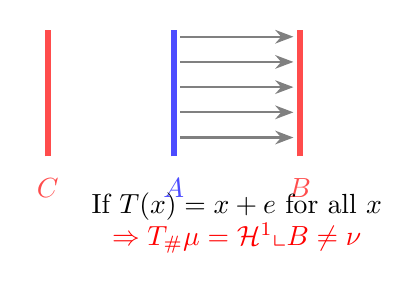
\begin{tikzpicture}[scale=0.8]
    % Segments
    \draw[red!70, line width=2pt] (-2,0) -- (-2,2);
    \node[red!70, below] at (-2,-0.2) {$C$};

    \draw[blue!70, line width=2pt] (0,0) -- (0,2);
    \node[blue!70, below] at (0,-0.2) {$A$};

    \draw[red!70, line width=2pt] (2,0) -- (2,2);
    \node[red!70, below] at (2,-0.2) {$B$};

    % All arrows going right (T = x + e)
    \foreach \y in {0.3, 0.7, 1.1, 1.5, 1.9} {
        \draw[-{Stealth}, gray, thick] (0.1, \y) -- (1.9, \y);
    }

    \node at (1, -0.8) {If $T(x) = x + e$ for all $x$};
    \node[red] at (1, -1.3) {$\Rightarrow T_\# \mu = \Hone \llcorner B \neq \nu$};
\end{tikzpicture}
\end{center}

$\Rightarrow$ \textbf{No optimal transport map exists!}
\end{frame}

%==============================================================================
\begin{frame}{Example 2: The Optimal Transport Plan}
\begin{columns}
\begin{column}{0.55\textwidth}
\textbf{Weak limit:} $\gamma_{T_n} \rightharpoonup \gamma^*$ where:
\[
\boxed{\gamma^* = \frac{1}{2}\gamma_{T^+} + \frac{1}{2}\gamma_{T^-}}
\]
with $T^{\pm}(x) = x \pm e$, $e = (1, 0)$.

\vspace{0.3cm}
\textbf{Properties:}
\begin{itemize}
    \item \textbf{Unique} optimal plan
    \item Cost $= 1$ (minimum)
    \item Not map-induced (splits!)
\end{itemize}
\end{column}
\begin{column}{0.45\textwidth}
\begin{center}
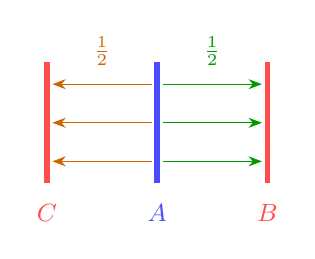
\begin{tikzpicture}[scale=0.7]
    % Segments
    \draw[red!70, line width=2pt] (-2,0) -- (-2,2.2);
    \node[red!70, below, font=\small] at (-2,-0.2) {$C$};

    \draw[blue!70, line width=2pt] (0,0) -- (0,2.2);
    \node[blue!70, below, font=\small] at (0,-0.2) {$A$};

    \draw[red!70, line width=2pt] (2,0) -- (2,2.2);
    \node[red!70, below, font=\small] at (2,-0.2) {$B$};

    % Splitting arrows
    \foreach \y in {0.4, 1.1, 1.8} {
        \draw[-{Stealth}, green!60!black] (0.1, \y) -- (1.9, \y);
        \draw[-{Stealth}, orange!80!black] (-0.1, \y) -- (-1.9, \y);
    }

    \node[green!60!black, font=\footnotesize] at (1, 2.4) {$\frac{1}{2}$};
    \node[orange!80!black, font=\footnotesize] at (-1, 2.4) {$\frac{1}{2}$};
\end{tikzpicture}
\end{center}
\end{column}
\end{columns}
\end{frame}

%==============================================================================
\begin{frame}{Key Insight: Maps vs Plans}
\begin{center}
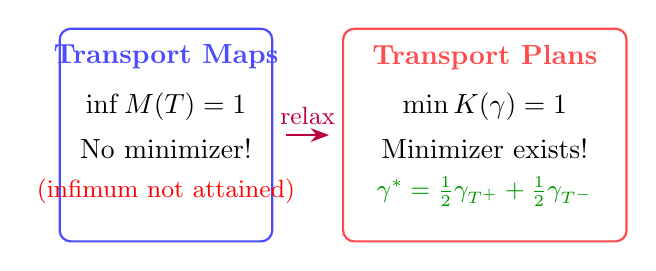
\begin{tikzpicture}[scale=0.9]
    % Box for maps
    \draw[blue!70, thick, rounded corners] (-3, -1.5) rectangle (0, 1.5);
    \node[blue!70, font=\bfseries] at (-1.5, 1.1) {Transport Maps};
    \node at (-1.5, 0.4) {$\inf M(T) = 1$};
    \node at (-1.5, -0.2) {No minimizer!};
    \node[red, font=\small] at (-1.5, -0.8) {(infimum not attained)};

    % Box for plans
    \draw[red!70, thick, rounded corners] (1, -1.5) rectangle (5, 1.5);
    \node[red!70, font=\bfseries] at (3, 1.1) {Transport Plans};
    \node at (3, 0.4) {$\min K(\gamma) = 1$};
    \node at (3, -0.2) {Minimizer exists!};
    \node[green!60!black, font=\small] at (3, -0.8) {$\gamma^* = \frac{1}{2}\gamma_{T^+} + \frac{1}{2}\gamma_{T^-}$};

    % Arrow
    \draw[-{Stealth}, thick, purple] (0.2, 0) -- node[above, font=\small] {relax} (0.8, 0);
\end{tikzpicture}
\end{center}

\vspace{0.4cm}
\textbf{Summary:}
\begin{itemize}
    \item $\inf$ among maps $=$ $\min$ among plans
    \item But the minimum may \textbf{not be achieved} by maps
    \item This motivates the \textbf{relaxation viewpoint}
\end{itemize}
\end{frame}

%==============================================================================
\section{Kantorovich as a Relaxation of Monge}
%==============================================================================

\begin{frame}{Rewriting the Monge Problem}
\textbf{Define:}
\[
K(\gamma) := \int_{\Omega \times \Omega} c \, d\gamma
\]

\vspace{0.3cm}
\textbf{Key observation:} For any transport map $T$:
\[
M(T) = \int_\Omega c(x, T(x)) \, d\mu(x) = \int_{\Omega \times \Omega} c \, d\gamma_T = K(\gamma_T)
\]

\vspace{0.3cm}
\textbf{Rewrite Monge Problem:}
\[
\boxed{\min\{J(\gamma) : \gamma \in \Pi(\mu, \nu)\}}
\]
where we define $J$ appropriately...
\end{frame}

%==============================================================================
\begin{frame}{The Functional $J$}
\textbf{Definition:}
\[
\boxed{J(\gamma) = \begin{cases}
K(\gamma) = M(T) & \text{if } \gamma = \gamma_T \text{ for some map } T \\
+\infty & \text{otherwise}
\end{cases}}
\]

\vspace{0.4cm}
\textbf{Interpretation:}
\begin{itemize}
    \item $J$ forces minimization over \textbf{map-induced plans only}
    \item Plans that split mass get infinite cost
\end{itemize}

\vspace{0.4cm}
\textbf{Now we can view (MP) and (KP) as:}
\begin{itemize}
    \item Same admissible set: $\Pi(\mu, \nu)$
    \item Different objectives: $J$ vs $K$
\end{itemize}
\end{frame}

%==============================================================================
\begin{frame}{Same Set, Different Functionals}
\begin{center}
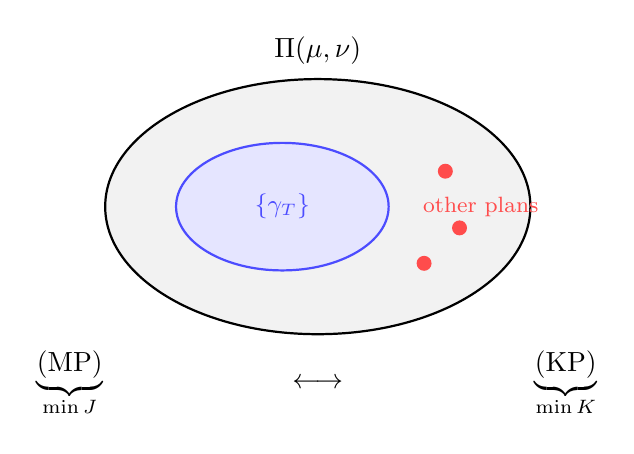
\begin{tikzpicture}[scale=0.9]
    % The set Pi
    \draw[thick, fill=gray!10] (0,0) ellipse (3 and 1.8);
    \node at (0, 2.2) {$\Pi(\mu, \nu)$};

    % Map-induced plans (subset)
    \draw[blue!70, thick, fill=blue!10] (-0.5, 0) ellipse (1.5 and 0.9);
    \node[blue!70, font=\small] at (-0.5, 0) {$\{\gamma_T\}$};

    % Other plans
    \fill[red!70] (1.8, 0.5) circle (3pt);
    \fill[red!70] (2, -0.3) circle (3pt);
    \fill[red!70] (1.5, -0.8) circle (3pt);
    \node[red!70, font=\footnotesize] at (2.3, 0) {other plans};

    % Labels below
    \node at (-3.5, -2.5) {$\underbrace{\text{(MP)}}_{\min J}$};
    \node at (0, -2.5) {$\longleftrightarrow$};
    \node at (3.5, -2.5) {$\underbrace{\text{(KP)}}_{\min K}$};
\end{tikzpicture}
\end{center}

\vspace{0.3cm}
\textbf{Question 1:} Why did Kantorovich replace $J$ with $K$?

\textbf{Question 2:} Can we prove that $\inf K = \inf J$?
\end{frame}

%==============================================================================
\begin{frame}{Box 1.10: Relaxation --- Definition}
\begin{block}{Definition (Relaxation)}
Let $F: X \to \R \cup \{+\infty\}$ be bounded from below on a metric space $X$.

The \textbf{relaxation} of $F$ is the functional $\overline{F}: X \to \R \cup \{+\infty\}$ defined as:
\[
\overline{F} := \sup\{G : G \leq F, \; G \text{ is l.s.c.}\}
\]
\end{block}

\vspace{0.3cm}
\textbf{Properties:}
\begin{itemize}
    \item $\overline{F}$ exists (supremum of l.s.c. functions is l.s.c.)
    \item $\overline{F}$ is the \textbf{maximal} l.s.c. functional with $\overline{F} \leq F$
    \item $\overline{F}$ is often called the \textbf{l.s.c. envelope} of $F$
\end{itemize}
\end{frame}

%==============================================================================
\begin{frame}{Relaxation: Representation Formula}
\begin{block}{Representation Formula}
\[
\boxed{\overline{F}(x) = \inf\left\{\liminf_{n \to \infty} F(x_n) : x_n \to x\right\}}
\]
\end{block}

\vspace{0.3cm}
\textbf{Proof idea:}
\begin{itemize}
    \item RHS is l.s.c. (by construction)
    \item RHS $\leq F$ (take constant sequence $x_n = x$)
    \item RHS is maximal with these properties
\end{itemize}

\vspace{0.3cm}
\textbf{Intuition:} $\overline{F}(x)$ = best cost you can achieve by \textbf{approaching} $x$.
\end{frame}

%==============================================================================
\begin{frame}{Key Property: $\inf F = \inf \overline{F}$}
\begin{block}{Theorem}
For any $F: X \to \R \cup \{+\infty\}$ bounded below:
\[
\boxed{\inf_X F = \inf_X \overline{F}}
\]
\end{block}

\vspace{0.3cm}
\textbf{Proof:}
\begin{enumerate}
    \item $F \geq \overline{F}$ $\Rightarrow$ $\inf F \geq \inf \overline{F}$

    \item For the reverse: Take any $x \in X$. By the representation formula:
    \[
    \overline{F}(x) = \inf\{\liminf_n F(x_n) : x_n \to x\} \geq \inf_X F
    \]

    \item Taking infimum over $x$: $\inf_X \overline{F} \geq \inf_X F$
\end{enumerate}

\vspace{0.2cm}
$\Rightarrow$ $\inf F = \inf \overline{F}$ \quad $\square$
\end{frame}

%==============================================================================
\begin{frame}{Relaxation: Visualization}
\begin{center}
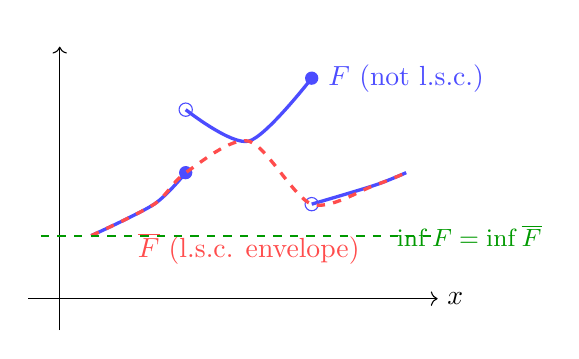
\begin{tikzpicture}[scale=0.8]
    % Axes
    \draw[->] (-0.5,0) -- (6,0) node[right] {$x$};
    \draw[->] (0,-0.5) -- (0,4) node[above] {};

    % Original function F (with jumps up)
    \draw[blue!70, very thick] plot[smooth] coordinates {(0.5, 1) (1.5, 1.5) (2, 2)};
    \fill[blue!70] (2, 2) circle (3pt);
    \fill[white] (2, 3) circle (3pt);
    \draw[blue!70] (2, 3) circle (3pt);
    \draw[blue!70, very thick] plot[smooth] coordinates {(2, 3) (3, 2.5) (4, 3.5)};
    \fill[blue!70] (4, 3.5) circle (3pt);
    \fill[white] (4, 1.5) circle (3pt);
    \draw[blue!70] (4, 1.5) circle (3pt);
    \draw[blue!70, very thick] plot[smooth] coordinates {(4, 1.5) (5, 1.8) (5.5, 2)};

    \node[blue!70] at (5.5, 3.5) {$F$ (not l.s.c.)};

    % Relaxation F-bar (l.s.c. envelope)
    \draw[red!70, very thick, dashed] plot[smooth] coordinates {(0.5, 1) (1.5, 1.5) (2, 2) (3, 2.5) (4, 1.5) (5, 1.8) (5.5, 2)};

    \node[red!70] at (3, 0.8) {$\overline{F}$ (l.s.c. envelope)};

    % Same infimum
    \draw[green!60!black, thick, dashed] (-0.3, 1) -- (6, 1);
    \node[green!60!black, font=\small] at (6.5, 1) {$\inf F = \inf \overline{F}$};
\end{tikzpicture}
\end{center}

\vspace{0.2cm}
\textbf{Key point:} Relaxation ``fills in'' the jumps downward, but preserves the infimum.
\end{frame}

%==============================================================================
\begin{frame}{Why This Matters for Optimal Transport}
\textbf{Claim:} $K = \overline{J}$ (relaxation of $J$)

\vspace{0.3cm}
\textbf{Why?}
\begin{itemize}
    \item $J$ is \textbf{NOT l.s.c.}: Map-induced plans $\{\gamma_T\}$ are not closed under weak limits
    \item $K$ \textbf{IS l.s.c.}: $K(\gamma) = \int c \, d\gamma$ is l.s.c. for weak convergence
    \item $K \leq J$: For $\gamma = \gamma_T$, we have $K(\gamma) = J(\gamma)$
    \item $K$ is maximal: Any l.s.c. $G \leq J$ satisfies $G \leq K$
\end{itemize}

\vspace{0.4cm}
\textbf{Therefore:}
\[
\boxed{\inf(\text{MP}) = \inf J = \inf \overline{J} = \inf K = \min(\text{KP})}
\]
\end{frame}

%==============================================================================
\begin{frame}{Summary: The Relaxation Viewpoint}
\begin{center}
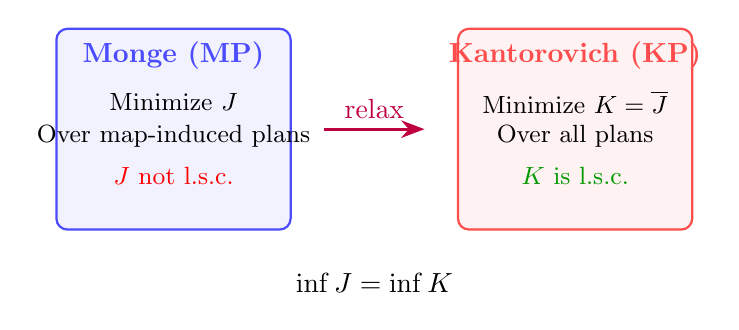
\begin{tikzpicture}[scale=0.85]
    % Monge box
    \draw[blue!70, thick, rounded corners, fill=blue!5] (-4, -1.5) rectangle (-0.5, 1.5);
    \node[blue!70, font=\bfseries] at (-2.25, 1.1) {Monge (MP)};
    \node[font=\small] at (-2.25, 0.4) {Minimize $J$};
    \node[font=\small] at (-2.25, -0.1) {Over map-induced plans};
    \node[red, font=\small] at (-2.25, -0.7) {$J$ not l.s.c.};

    % Arrow
    \draw[-{Stealth}, very thick, purple] (0, 0) -- node[above] {relax} (1.5, 0);

    % Kantorovich box
    \draw[red!70, thick, rounded corners, fill=red!5] (2, -1.5) rectangle (5.5, 1.5);
    \node[red!70, font=\bfseries] at (3.75, 1.1) {Kantorovich (KP)};
    \node[font=\small] at (3.75, 0.4) {Minimize $K = \overline{J}$};
    \node[font=\small] at (3.75, -0.1) {Over all plans};
    \node[green!60!black, font=\small] at (3.75, -0.7) {$K$ is l.s.c.};

    % Same infimum
    \node at (0.75, -2.3) {$\inf J = \inf K$};
\end{tikzpicture}
\end{center}

\vspace{0.3cm}
\textbf{Kantorovich's genius:}
\begin{itemize}
    \item Replace non-l.s.c. functional $J$ with its relaxation $K$
    \item \textbf{Same infimum}, but $K$ has minimizers (by Weierstrass!)
    \item Optimal plans = limit points of approximately optimal maps
\end{itemize}
\end{frame}

%==============================================================================
\section{Exercises}
%==============================================================================

\begin{frame}{Exercise 1: Dirac Mass Transport}
\textbf{Problem:} Let $\mu = \delta_0$ and $\nu = \frac{1}{3}\delta_{-1} + \frac{1}{3}\delta_0 + \frac{1}{3}\delta_1$ on $\R$.

Cost: $c(x,y) = |x-y|^2$.

\vspace{0.4cm}
\textbf{Questions:}
\begin{enumerate}
    \item[(a)] Does a transport map $T$ with $T_\# \mu = \nu$ exist?
    \item[(b)] Find the unique transport plan $\gamma \in \Pi(\mu, \nu)$.
    \item[(c)] Compute the transport cost $\int c \, d\gamma$.
\end{enumerate}

\vspace{0.4cm}
\textit{Hint:} Recall that $T_\# \delta_a = \delta_{T(a)}$ and $\Pi(\delta_a, \nu) = \{\delta_a \otimes \nu\}$.
\end{frame}

%==============================================================================
\begin{frame}{Solution 1}
\begin{columns}
\begin{column}{0.5\textwidth}
\textbf{(a)} No transport map exists.

$T_\# \delta_0 = \delta_{T(0)}$ (always Dirac).

But $\nu$ has 3 atoms $\Rightarrow$ impossible.

\vspace{0.2cm}
\textbf{(b)} Unique transport plan:
\[
\gamma = \delta_0 \otimes \nu
\]
\[
= \tfrac{1}{3}\delta_{(0,-1)} + \tfrac{1}{3}\delta_{(0,0)} + \tfrac{1}{3}\delta_{(0,1)}
\]

\vspace{0.2cm}
\textbf{(c)} Cost $= \frac{1}{3}(1+0+1) = \boxed{\frac{2}{3}}$
\end{column}
\begin{column}{0.5\textwidth}
\begin{center}
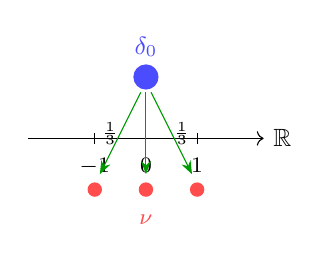
\begin{tikzpicture}[scale=0.65]
    % Number line
    \draw[->] (-2.3,0) -- (2.3,0) node[right] {\small $\R$};
    \foreach \x in {-1,0,1} {
        \draw (\x, 0.1) -- (\x, -0.1);
        \node[below, font=\footnotesize] at (\x, -0.2) {$\x$};
    }

    % Source
    \fill[blue!70] (0, 1.2) circle (7pt);
    \node[above, blue!70, font=\small] at (0, 1.4) {$\delta_0$};

    % Targets
    \fill[red!70] (-1, -1) circle (4pt);
    \fill[red!70] (0, -1) circle (4pt);
    \fill[red!70] (1, -1) circle (4pt);
    \node[below, red!70, font=\footnotesize] at (0, -1.3) {$\nu$};

    % Splitting arrows
    \draw[-{Stealth}, green!60!black] (-0.1, 0.9) -- (-0.9, -0.7);
    \draw[-{Stealth}, green!60!black] (0, 0.9) -- (0, -0.7);
    \draw[-{Stealth}, green!60!black] (0.1, 0.9) -- (0.9, -0.7);

    \node[font=\tiny] at (-0.7, 0.1) {$\frac{1}{3}$};
    \node[font=\tiny] at (0.7, 0.1) {$\frac{1}{3}$};
\end{tikzpicture}

\vspace{0.2cm}
\textbf{Cost breakdown:}
\begin{itemize}
    \item $(0,-1)$: $|0-(-1)|^2 = 1$
    \item $(0,0)$: $|0-0|^2 = 0$
    \item $(0,1)$: $|0-1|^2 = 1$
\end{itemize}
\end{center}
\end{column}
\end{columns}
\end{frame}

%==============================================================================
\begin{frame}{Exercise 2: Three Segments Problem}
\textbf{Problem:} Using the setup from Example 2 (segments $A$, $B$, $C$):

\vspace{0.3cm}
\begin{enumerate}
    \item[(a)] For $n = 2$, write the formula for $T_2$ explicitly.

    \vspace{0.2cm}
    \item[(b)] Compute $\text{Cost}(T_2)$ (you may leave as an integral).

    \vspace{0.2cm}
    \item[(c)] Verify that $\gamma^* = \frac{1}{2}\gamma_{T^+} + \frac{1}{2}\gamma_{T^-}$ satisfies the marginal constraints, i.e., $\gamma^* \in \Pi(\mu, \nu)$.
\end{enumerate}

\vspace{0.4cm}
\textit{Hint:} For (c), check that projecting $\gamma^*$ onto the first coordinate gives $\mu$, and onto the second gives $\nu$.
\end{frame}

%==============================================================================
\begin{frame}{Solution 2 (Part a)}
\textbf{(a)} For $n = 2$: $A$ divided into 4 segments, $B$ and $C$ into 2 each.

\vspace{0.2cm}
\begin{center}
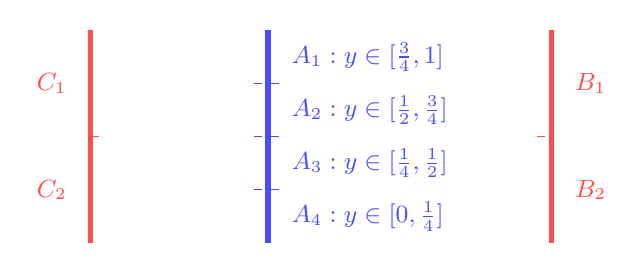
\begin{tikzpicture}[scale=0.9]
    % Segment C
    \draw[red!70, line width=2pt] (-2.5,0) -- (-2.5,3);
    \draw[red!70, dashed] (-2.5,1.5) -- (-2.3,1.5);
    \node[red!70, left, font=\small] at (-2.7,2.25) {$C_1$};
    \node[red!70, left, font=\small] at (-2.7,0.75) {$C_2$};

    % Segment A
    \draw[blue!70, line width=2pt] (0,0) -- (0,3);
    \foreach \y in {0.75, 1.5, 2.25} {
        \draw[blue!70, dashed] (-0.2,\y) -- (0.2,\y);
    }
    \node[blue!70, right, font=\small] at (0.2,2.625) {$A_1: y \in [\frac{3}{4}, 1]$};
    \node[blue!70, right, font=\small] at (0.2,1.875) {$A_2: y \in [\frac{1}{2}, \frac{3}{4}]$};
    \node[blue!70, right, font=\small] at (0.2,1.125) {$A_3: y \in [\frac{1}{4}, \frac{1}{2}]$};
    \node[blue!70, right, font=\small] at (0.2,0.375) {$A_4: y \in [0, \frac{1}{4}]$};

    % Segment B
    \draw[red!70, line width=2pt] (4,0) -- (4,3);
    \draw[red!70, dashed] (3.8,1.5) -- (4,1.5);
    \node[red!70, right, font=\small] at (4.2,2.25) {$B_1$};
    \node[red!70, right, font=\small] at (4.2,0.75) {$B_2$};
\end{tikzpicture}
\end{center}

\vspace{0.2cm}
$T_2$: piecewise affine, $A_1 \to B_1$, $A_2 \to C_1$, $A_3 \to B_2$, $A_4 \to C_2$
\end{frame}

%==============================================================================
\begin{frame}{Solution 2 (Parts b-c)}
\textbf{(b)} $\text{Cost}(T_2)$:

Each segment $A_i$ has length $\frac{1}{4}$, mapped to target of length $\frac{1}{2}$.

Horizontal displacement $= 1$, vertical displacement $\leq \frac{1}{4}$.
\[
\text{Cost}(T_2) = \int_A |T_2(x) - x|^2 \, d\Hone < 1 + \frac{1}{4} \cdot \frac{1}{4} = 1 + \frac{1}{16}
\]

\vspace{0.3cm}
\textbf{(c)} Marginal check for $\gamma^* = \frac{1}{2}\gamma_{T^+} + \frac{1}{2}\gamma_{T^-}$:

\textbf{First marginal:}
\[
(\pi_x)_\# \gamma^* = \frac{1}{2}(\pi_x)_\# \gamma_{T^+} + \frac{1}{2}(\pi_x)_\# \gamma_{T^-} = \frac{1}{2}\mu + \frac{1}{2}\mu = \mu \quad \checkmark
\]

\textbf{Second marginal:}
\[
(\pi_y)_\# \gamma^* = \frac{1}{2}(T^+)_\# \mu + \frac{1}{2}(T^-)_\# \mu = \frac{1}{2}\Hone \llcorner B + \frac{1}{2}\Hone \llcorner C = \nu \quad \checkmark
\]
\end{frame}

%==============================================================================
\section{Summary}
%==============================================================================

\begin{frame}{Summary}
\textbf{Counter-example 1: No Transport Map Exists}
\begin{itemize}
    \item $\mu = \delta_a$ (Dirac mass) $\Rightarrow$ $T_\# \delta_a = \delta_{T(a)}$
    \item Cannot transport to non-Dirac $\nu$ via maps
    \item Kantorovich: $\gamma = \delta_a \otimes \nu$ solves (KP)
\end{itemize}

\vspace{0.3cm}
\textbf{Counter-example 2: Maps Exist but No Optimal Map}
\begin{itemize}
    \item Three segments $A, B, C$ with $\mu = \Hone \llcorner A$, $\nu = \frac{1}{2}(\Hone \llcorner B + \Hone \llcorner C)$
    \item $\inf M(T) = 1$, but no map achieves it
    \item Optimal plan: $\gamma^* = \frac{1}{2}\gamma_{T^+} + \frac{1}{2}\gamma_{T^-}$ with cost $1$
\end{itemize}

\vspace{0.3cm}
\textbf{Relaxation Viewpoint}
\begin{itemize}
    \item $K = \overline{J}$ (l.s.c. relaxation of $J$)
    \item $\inf(\text{MP}) = \inf J = \inf K = \min(\text{KP})$
    \item Kantorovich finds minimizers even when Monge cannot
\end{itemize}
\end{frame}

\end{document}
